\documentclass[hyperref=colorlinks]{beamer}
\mode<presentation>
\usetheme{iclpt}
\setbeamertemplate{navigation symbols}{}
\setbeamertemplate{headline}{
  \begin{beamercolorbox}[leftskip=.2cm,rightskip=.2cm,topskip=.2cm,ht=1.1cm,dp=0.1cm,wd=\textwidth]{institute in head/foot}
    
\includegraphics[height=1cm]{icl.pdf}
    \hfill
    
\includegraphics[height=1cm]{../Pics/CMS-Color.pdf}
  \end{beamercolorbox}
}
\setbeamertemplate{footline}{
  \begin{beamercolorbox}[ht=.35cm,dp=0.2cm,wd=\textwidth,leftskip=.3cm]{author in head/foot}%
    \begin{minipage}[c]{5cm}%
      \usebeamerfont{author in head/foot}
      \insertshortauthor 
      \insertshorttitle
    \end{minipage}\hfill%
    \hfill
    \insertframenumber{} / \ref{lastframe}
    %\hfill
    \begin{minipage}{6cm}
      \hfill
      %\insertshorttitle
    \end{minipage}
  \end{beamercolorbox}%
}

\definecolor{beamer@icdarkblue}{RGB}{0,51,102}
\definecolor{beamer@icmiddleblue}{RGB}{0,82,150} 
\definecolor{beamer@iclightblue}{RGB}{200,212,232}
\definecolor{beamer@icmiddlered}{RGB}{204,51,0}
\definecolor{beamer@iclightred}{RGB}{232,212,32}

\usepackage{tikz}
\usetikzlibrary{arrows,shapes,backgrounds}
\usepackage{color}
\usepackage{tabularx,colortbl}
\usepackage{graphicx}
\usepackage{pdfpages}
\usepackage{feynmp}
\usepackage{rotating}
\usepackage{moresize}
\usepackage{slashed}
\usepackage{xcolor,colortbl}
\DeclareGraphicsRule{*}{mps}{*}{}
\hypersetup{colorlinks=false}

\title[Invisible Higgs at CMS]{\vspace{-0.2cm} Searching for the Higgs boson at the LHC}
\author[P. Dunne]{\underline{P. Dunne} - Imperial College London} % A.M. Magnan and A. Nikitenko Joao Pela with \\ R. Aggleton, J. Brooke: Bristol \\ C.Asawangtrakuldee, Q.Li: Peking \\ P. Srimanobhas: Chulalongkorn \\ S. Kumar, K. Mazumdar: Mumbai}
\titlegraphic{
  \vspace{-0.7cm}
  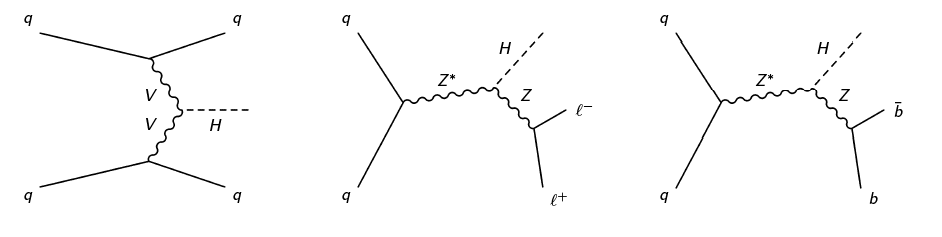
\includegraphics[width=\textwidth]{TalkPics/invcomb021213/feyndiags}
  %% \begin{fmfgraph*}(100,70)
  %%         \fmfleft{i1,i2}
  %%         \fmfright{o1,o2,o3}
  %%         \fmf{fermion}{i1,v1,o1}
  %%         \fmf{fermion}{i2,v2,o3}
  %%         \fmf{phantom,tension=4/5}{v1,v2}
  %%         \fmffreeze
  %%         \fmf{photon,label=$W,,Z$}{v1,v3}
  %%         \fmf{photon,label=$W,,Z$}{v2,v3}
  %%         \fmf{dashes}{v3,o2}
  %%         \fmflabel{$q$}{i1}
  %%         \fmflabel{$q$}{i2}
  %%         \fmflabel{$q$}{o1}
  %%         \fmflabel{$q$}{o3}
  %%         \fmflabel{$H$}{o2}

  %%       \end{fmfgraph*}
}
\date{}
\begin{document}
\tikzstyle{every picture}+=[remember picture]
\tikzstyle{na} = [baseline=-.5ex]
\begin{fmffile}{sgsfeyndiags}

  %TITLE PAGE
  \section{Title}
  \begin{frame}
    \titlepage
    
  \end{frame}

  \begin{frame}
    \frametitle{Introduction}
    \begin{itemize}
    \item What is the LHC?
    \item What is the Higgs boson?
    \item How do we search for it?
    \item What do we see?
    \end{itemize}
  \end{frame}

  %!!MORE DETAIL ON LHC AND CMS
  \begin{frame}
    \frametitle{CMS and the LHC}
    \begin{center}
      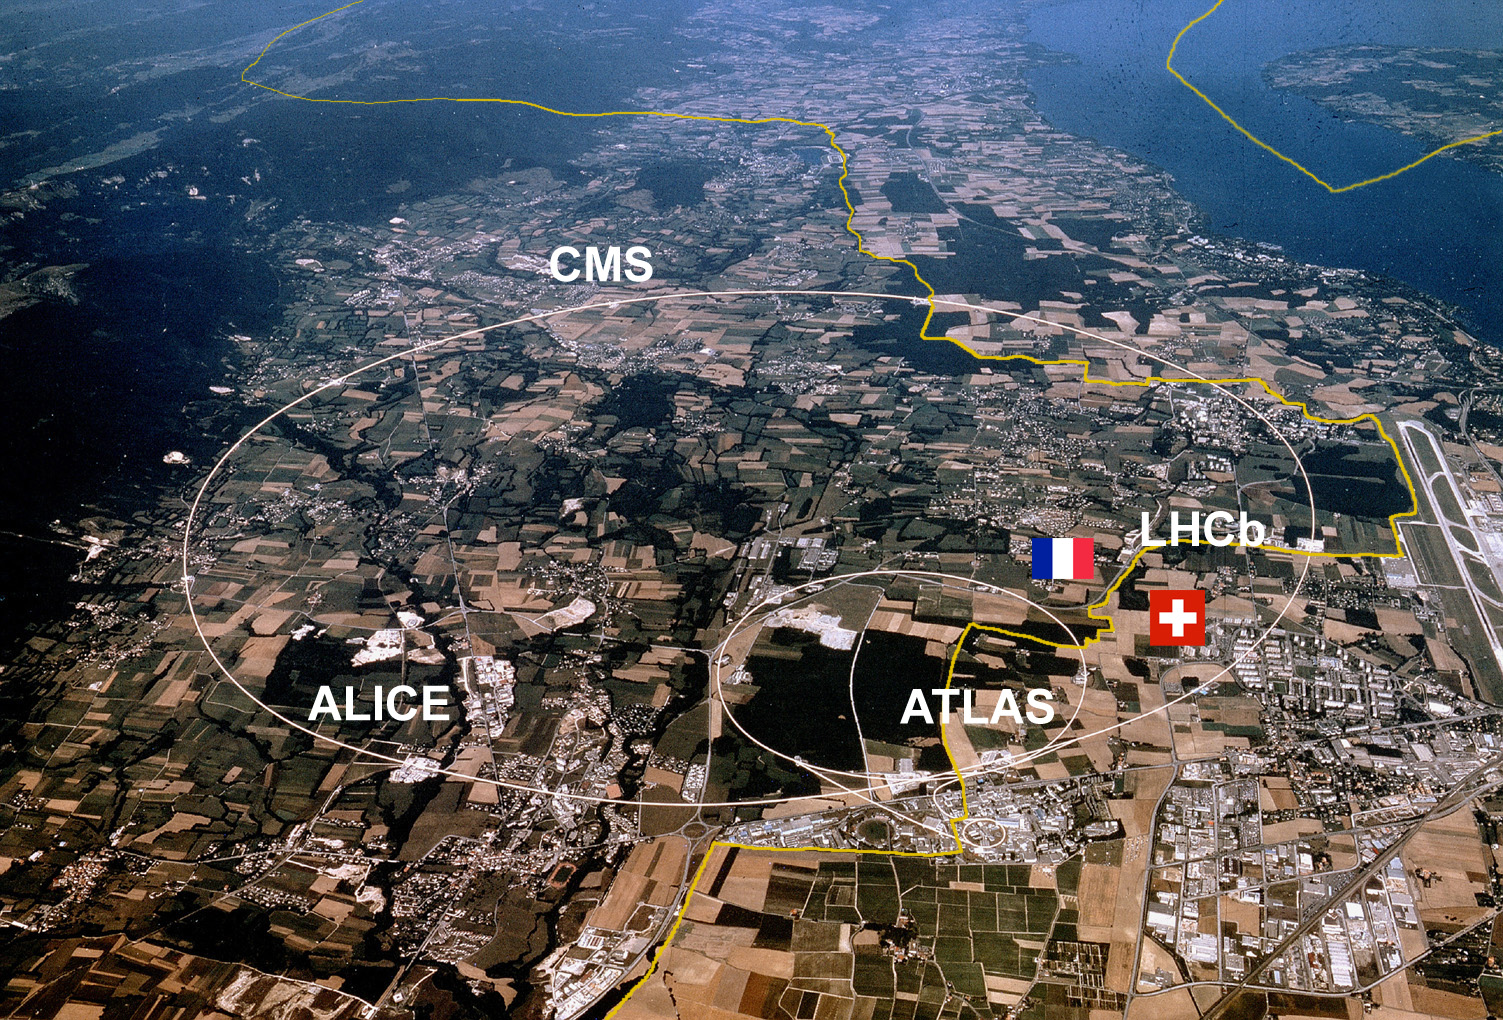
\includegraphics[width=.9\textwidth]{TalkPics/cern-lhc-aerial.jpg}
    \end{center}
  \end{frame}
  
  \begin{frame}
    \frametitle{CMS and the LHC}
    \begin{center}
      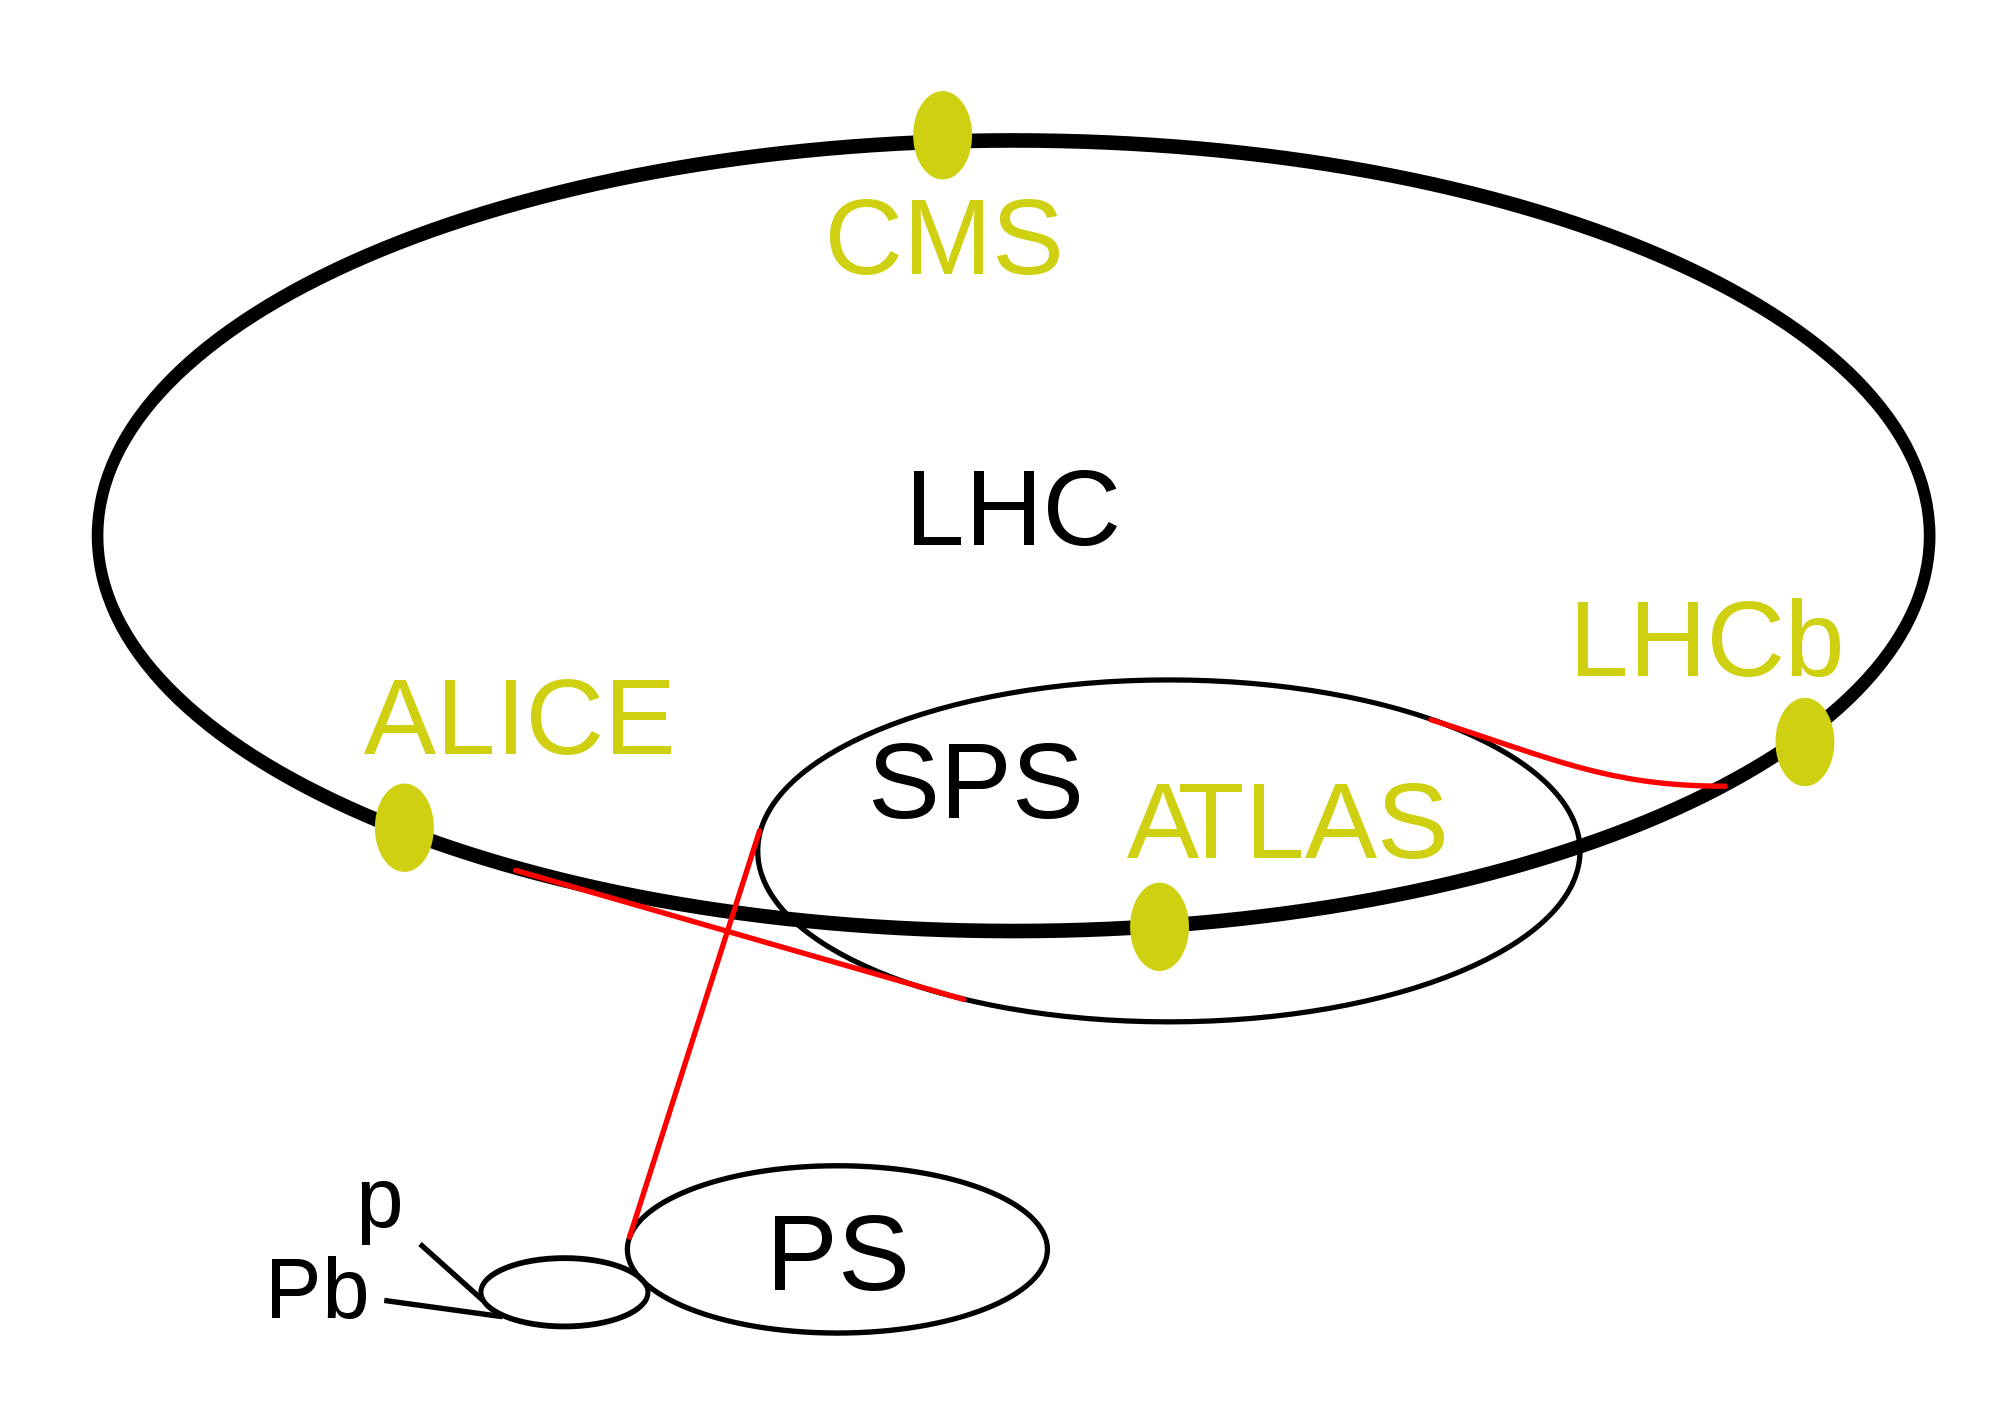
\includegraphics[width=.9\textwidth]{TalkPics/sgs120315/acceleratorchain.png}
      \end{center}
  \end{frame}

    \begin{frame}
    \frametitle{CMS}
    \centering
    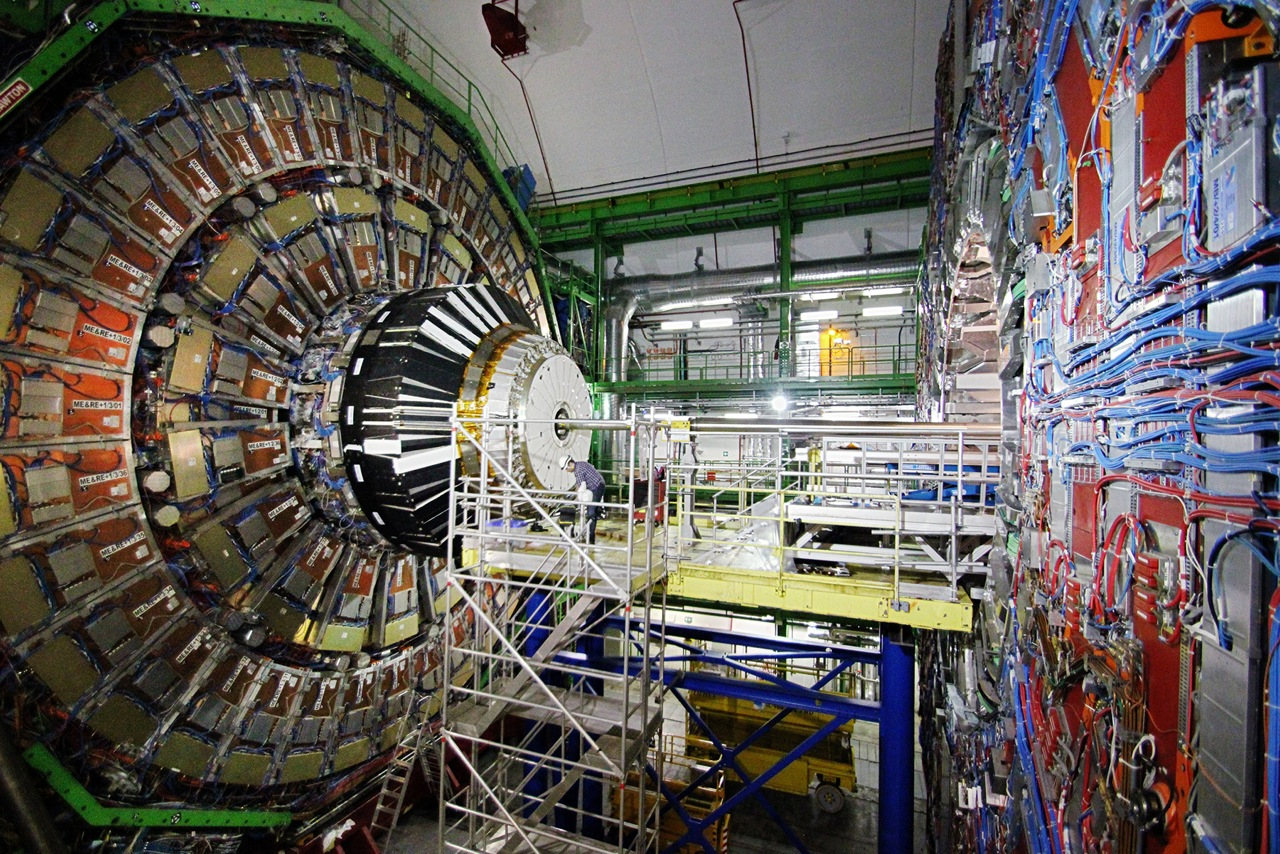
\includegraphics[height=.85\textheight]{TalkPics/sgs120315/cmsphoto.jpeg}
  \end{frame}

  \begin{frame}
    \frametitle{CMS}
    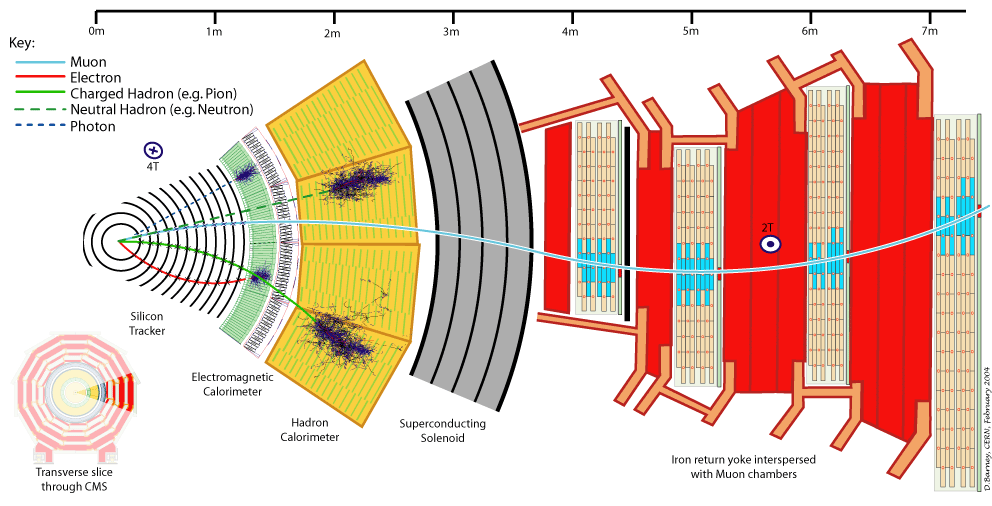
\includegraphics[width=\textwidth]{TalkPics/CMS_Slice.png}
  \end{frame}

  \begin{frame}
    \frametitle{Symmetry and the Standard Model (SM)}
    %!!EXPLAIN NOETHER'S THEOREM
    %!!EVERYTHING HAS TO BE SCALAR, USE VECTOR AS AN EXAMPLE
    \begin{itemize}
    \item[1)]<1-> The universe has symmetries:
      \begin{itemize}
        \color{beamer@icmiddleblue}
      \item<1-> Results of experiments are the same if the apparatus is in London or Lisbon
      \end{itemize}
    \item[2)]<2-> The equations that govern the universe must also have these symmetries:
      \begin{itemize}
        \color{beamer@icmiddleblue}
        \item<2-> Everything that can happen will so if the universe never breaks a symmetry it's a good hint of a fundamental property
      \end{itemize}
      
    \item[3)]<3-> Start by writing down the most general formula that satisfies the symmetries:
      \begin{itemize}
        \color{beamer@icmiddleblue}
        \item<3-> Need to know what particles you're trying to describe
      \end{itemize}
    \end{itemize}
  \end{frame}

  \begin{frame}
    \frametitle{SM Particles}
    \centering
    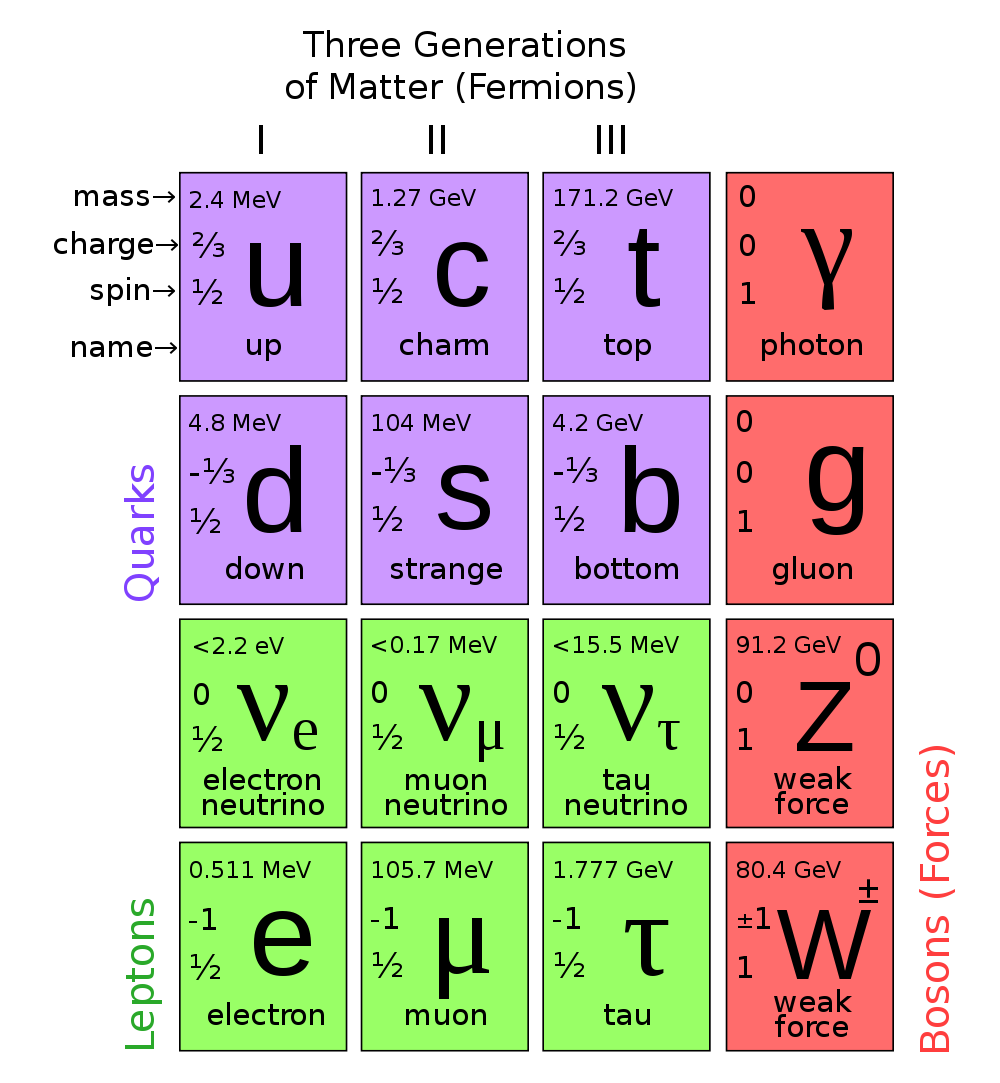
\includegraphics[height=.8\textheight]{TalkPics/sgs120315/SM.png}
  \end{frame}

  \begin{frame}
    \frametitle{The Higgs boson}
    \begin{columns}
      \column{.5\textwidth}
      \begin{itemize}
        \color{beamer@icmiddleblue}
      \item<1-> Things have mass
      \item<2-> Mass terms for particles/forces we know about break symmetries
      \item<3-> There must be another particle/force with exactly the properties to give things mass
      \end{itemize}
      \column{.5\textwidth}
      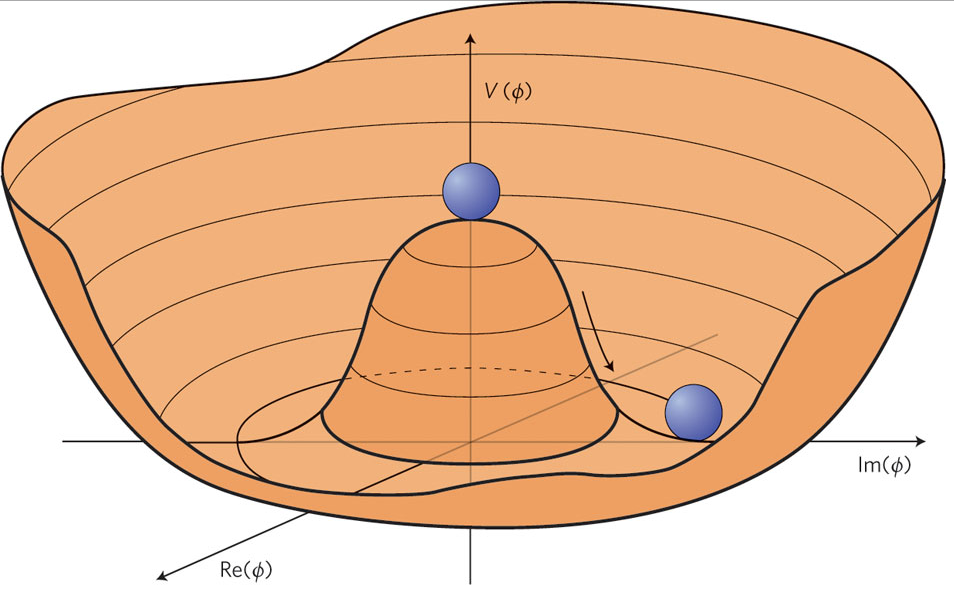
\includegraphics[width=\textwidth]{TalkPics/sgs120315/higgspotential.png}
    \end{columns}
  \end{frame}



  \begin{frame}
    \frametitle{Symmetry and the SM}
    \begin{columns}
      \column{1.1\textwidth}
    \begin{itemize}
    \item \tikz[na] \node (forces) {Forces: EM, strong, weak};
    \end{itemize}
    
    \tikzstyle{na} = [baseline=-.5ex]
    \begin{align*}
      \tikz[baseline]{
        \node[anchor=base] (L){$\mathcal{L} =$};
      }
      \tikz[baseline]{
        \node[anchor=base,fill=blue!20] (kinetics){$-\frac{1}{4}F_{\mu\nu}F^{\mu\nu}+i\bar{\psi}\slashed{D}\psi + h.c.$};
      } +
      \tikz[baseline]{
        \node[anchor=base,fill=red!20] (fermionmass){$ \bar{\psi}_{i}y_{ij}\psi_{j}\phi+h.c.$};
      }+
      \tikz[baseline]{
        \node[anchor=base,fill=green!20] (bosonmass){$|D_{\mu}\phi|^2-V(\phi)$};
      }
    \end{align*}
    \begin{itemize}
    \item \tikz[na] \node (masses) {Quark and lepton Masses};
    \item \tikz[na] \node (higgs) {Boson masses and Higgs potential};
    \end{itemize}

    \begin{tikzpicture}[overlay]
      \path[->] (forces) edge [color=blue,very thick] (kinetics);
      \path[->] (masses.east) edge [color=red,very thick] (fermionmass);
      \path[->] (higgs.east) edge [color=green,very thick] (bosonmass);
    \end{tikzpicture}
    \end{columns}
  \end{frame}

  \begin{frame}
    \frametitle{How is the Higgs made at the LHC?}
    \begin{columns}
      \column{.33\textwidth}
    \begin{block}{ggH}
      \vspace{.5cm}
      \hspace{.1cm}
      \begin{fmfgraph*}(80,70)
        \fmfleft{i1,i2}
        \fmfright{f1,o1,f2}
        \fmf{gluon,tension=7/5}{i1,v1}
        \fmf{gluon,tension=7/5}{i2,v2}
        \fmf{phantom}{v1,f1}
        \fmf{phantom}{v2,f2}
        \fmf{phantom}{v1,v2}
        \fmffreeze
        \fmf{fermion}{v1,v2,v3,v1}
        \fmf{dashes,tension=6/5}{v3,o1}
        \fmflabel{$g$}{i1}
        \fmflabel{$g$}{i2}
        \fmflabel{$H$}{o1}
      \end{fmfgraph*}
      \vspace{.4cm}
      \end{block}
      \column{.33\textwidth}
      \begin{block}{VBF}
      \vspace{.5cm}
      \begin{fmfgraph*}(80,70)
        \fmfleft{i1,i2}
        \fmfright{o1,o2,o3}
        \fmf{fermion}{i1,v1,o1}
        \fmf{fermion}{i2,v2,o3}
        \fmf{phantom,tension=4/5}{v1,v2}
        \fmffreeze
        \fmf{photon,label=$W,,Z$}{v1,v3}
        \fmf{photon,label=$W,,Z$}{v2,v3}
        \fmf{dashes}{v3,o2}
        \fmflabel{$q$}{i1}
        \fmflabel{$q$}{i2}
        \fmflabel{$q$}{o1}
        \fmflabel{$q$}{o3}
        \fmflabel{$H$}{o2}
      \end{fmfgraph*}
      \vspace{.4cm}
      \end{block}
      \column{.33\textwidth}
      \begin{block}{Z/WH}
      \vspace{.5cm}
      \begin{fmfgraph*}(80,70)
        \fmfleft{i1,i2}
        \fmfright{o1,o2}
        \fmf{fermion}{i1,v1,i2}
        \fmf{photon,label=$W,,Z$}{v1,v2}
        \fmf{photon}{v2,o1}
        \fmf{dashes}{v2,o2}
        \fmflabel{$q$}{i1}
        \fmflabel{$q$}{i2}
        \fmflabel{$H$}{o2}
        \fmflabel{$W,Z$}{o1}
      \end{fmfgraph*}
      \vspace{.4cm}
      \end{block}
      \end{columns}
  \end{frame}

  \begin{frame}
    \frametitle{What does the Higgs boson look like at the LHC?}
      \includegraphics[width=.5\textwidth,height=.55\textwidth,clip=true,trim=0 0 0 0]{../../Reports/Firstyearreport/Higgs_XS_8TeV_lx.pdf}
      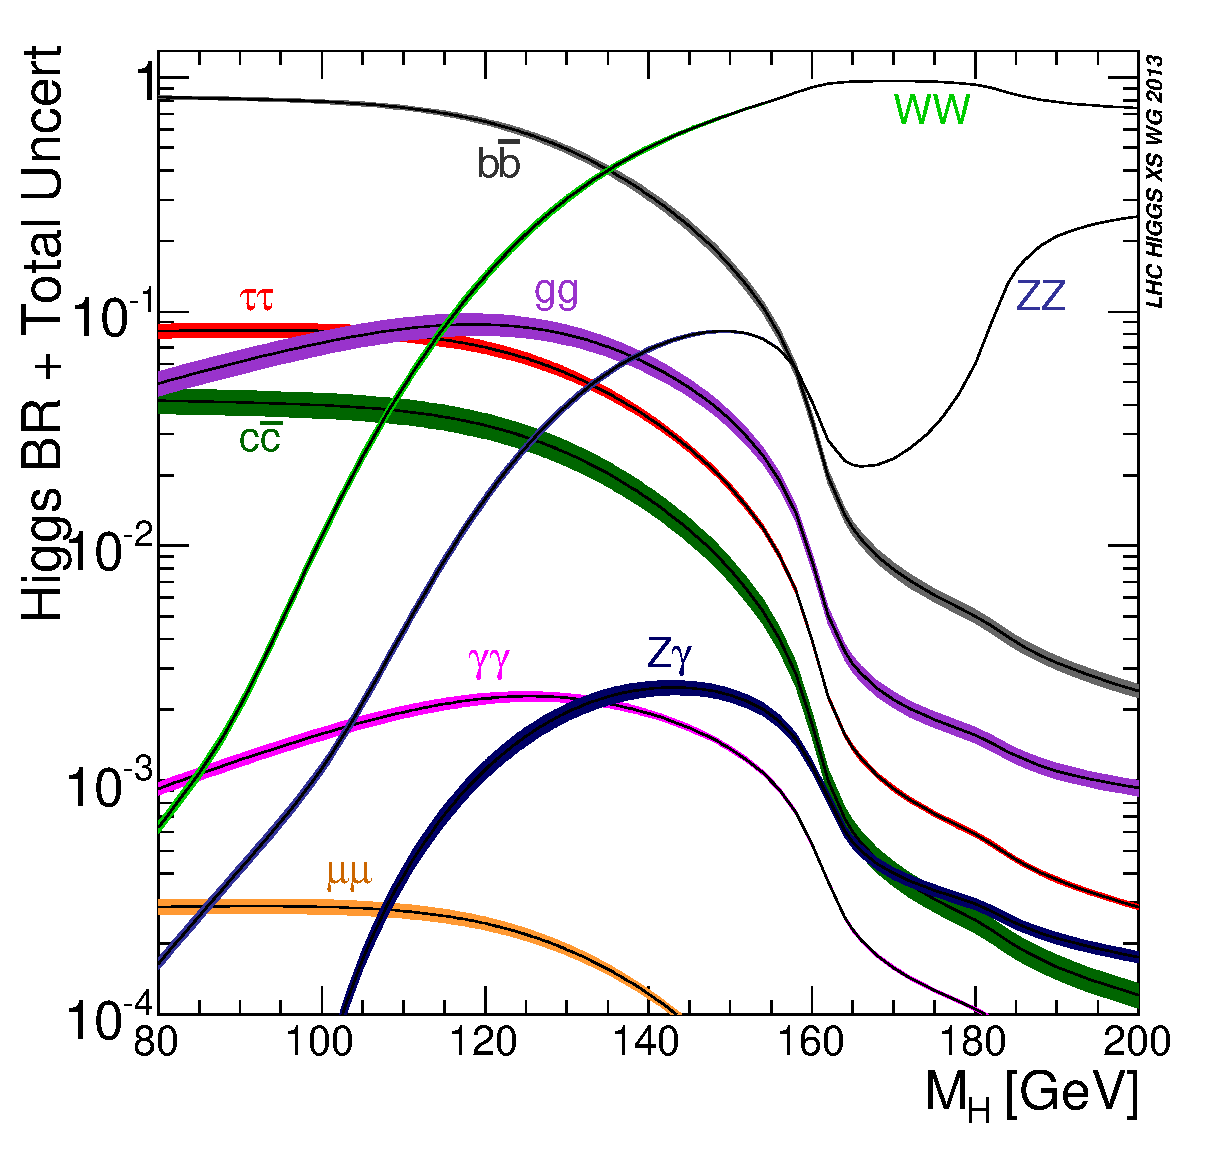
\includegraphics[width=.5\textwidth,height=.55\textwidth,clip=true,trim=0 10 0 10]{TalkPics/sgs120315/Higgs_BR_LM.eps}
  \end{frame}


  \begin{frame}
    \frametitle{Getting the data}
    %TRIGGERING
    \begin{columns}
      \column{1.1\textwidth}
    \begin{tikzpicture}
      \node (l1node){
        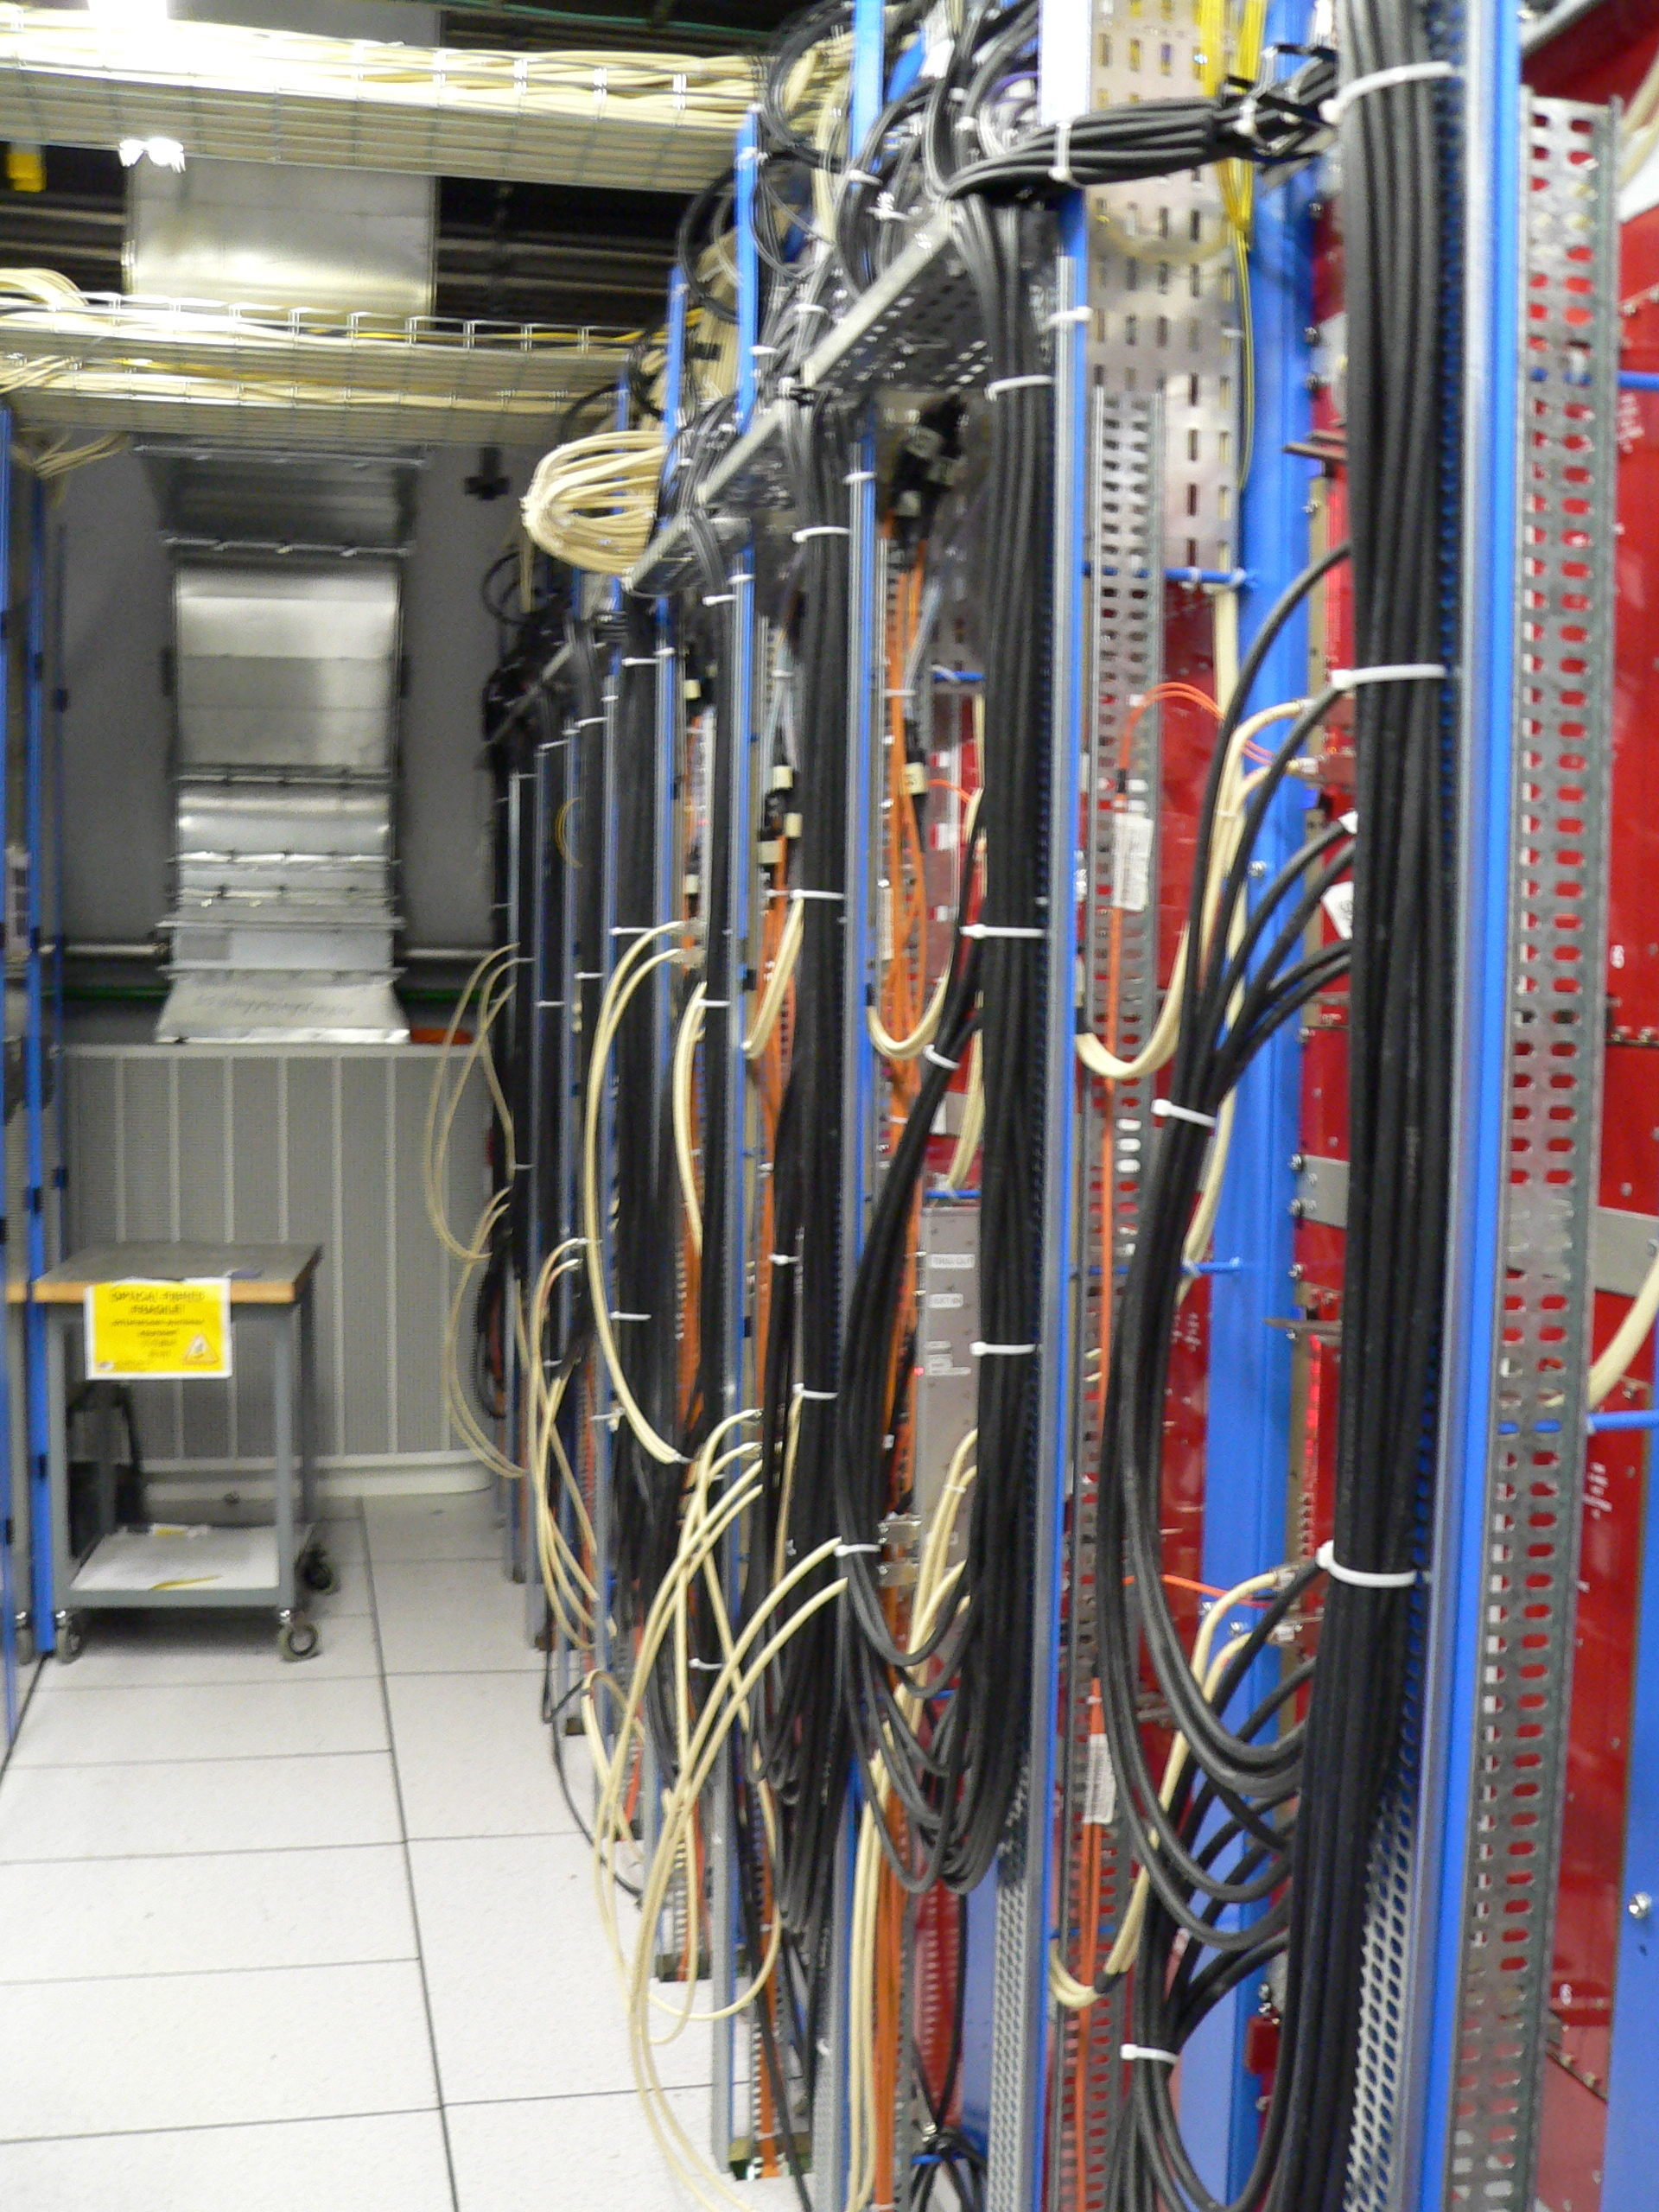
\includegraphics[width=.3\textwidth]{TalkPics/sgs120315/L1.jpg}
      };
      \node[node distance=4cm,right of=l1node] (hltnode){
        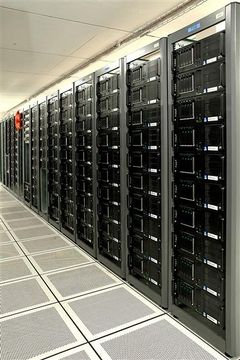
\includegraphics[width=.3\textwidth]{TalkPics/sgs120315/HLT.jpg}
      };
      \node[node distance=4cm,right of=hltnode] (gridnode){
        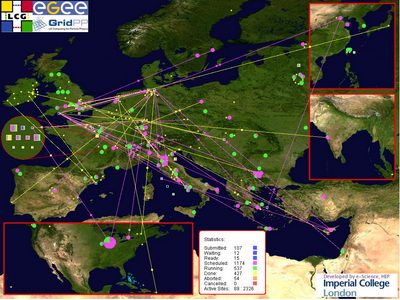
\includegraphics[width=.3\textwidth]{TalkPics/sgs120315/grid.jpg}
      };
      \node at (l1node.north) {\color{beamer@icmiddleblue}{Level 1 Trigger}};
      \node at (hltnode.north) {\color{beamer@icmiddleblue}{High Level Trigger}};
      \node at (gridnode.north) {\color{beamer@icmiddleblue}{Analysis}};
      \node at (l1node.south) {\color{beamer@icmiddleblue}{40MHz $\rightarrow$ 100kHz}};
      \node at (hltnode.south) {\color{beamer@icmiddleblue}{100kHz $\rightarrow$ 1kHz}};
      \path[->,color=red,very thick] (1.4,0.3) edge (2.4,0.3);
      \path[->,color=red,very thick] (5.4,0.3) edge (6.4,0.3);
    \end{tikzpicture}
    \end{columns}
    
  \end{frame}

  %!!DOING ANALYSIS ONE DIST HOW YOU MIGHT CUT, THEN LOTS TO SHOW BIG DATA ASPECT
  %!!SOME RESULTS

  \begin{frame}
    \frametitle{How do we search for it?}
    \begin{itemize}
    \item Pick a region with lots of signal and not much background
    \end{itemize}
    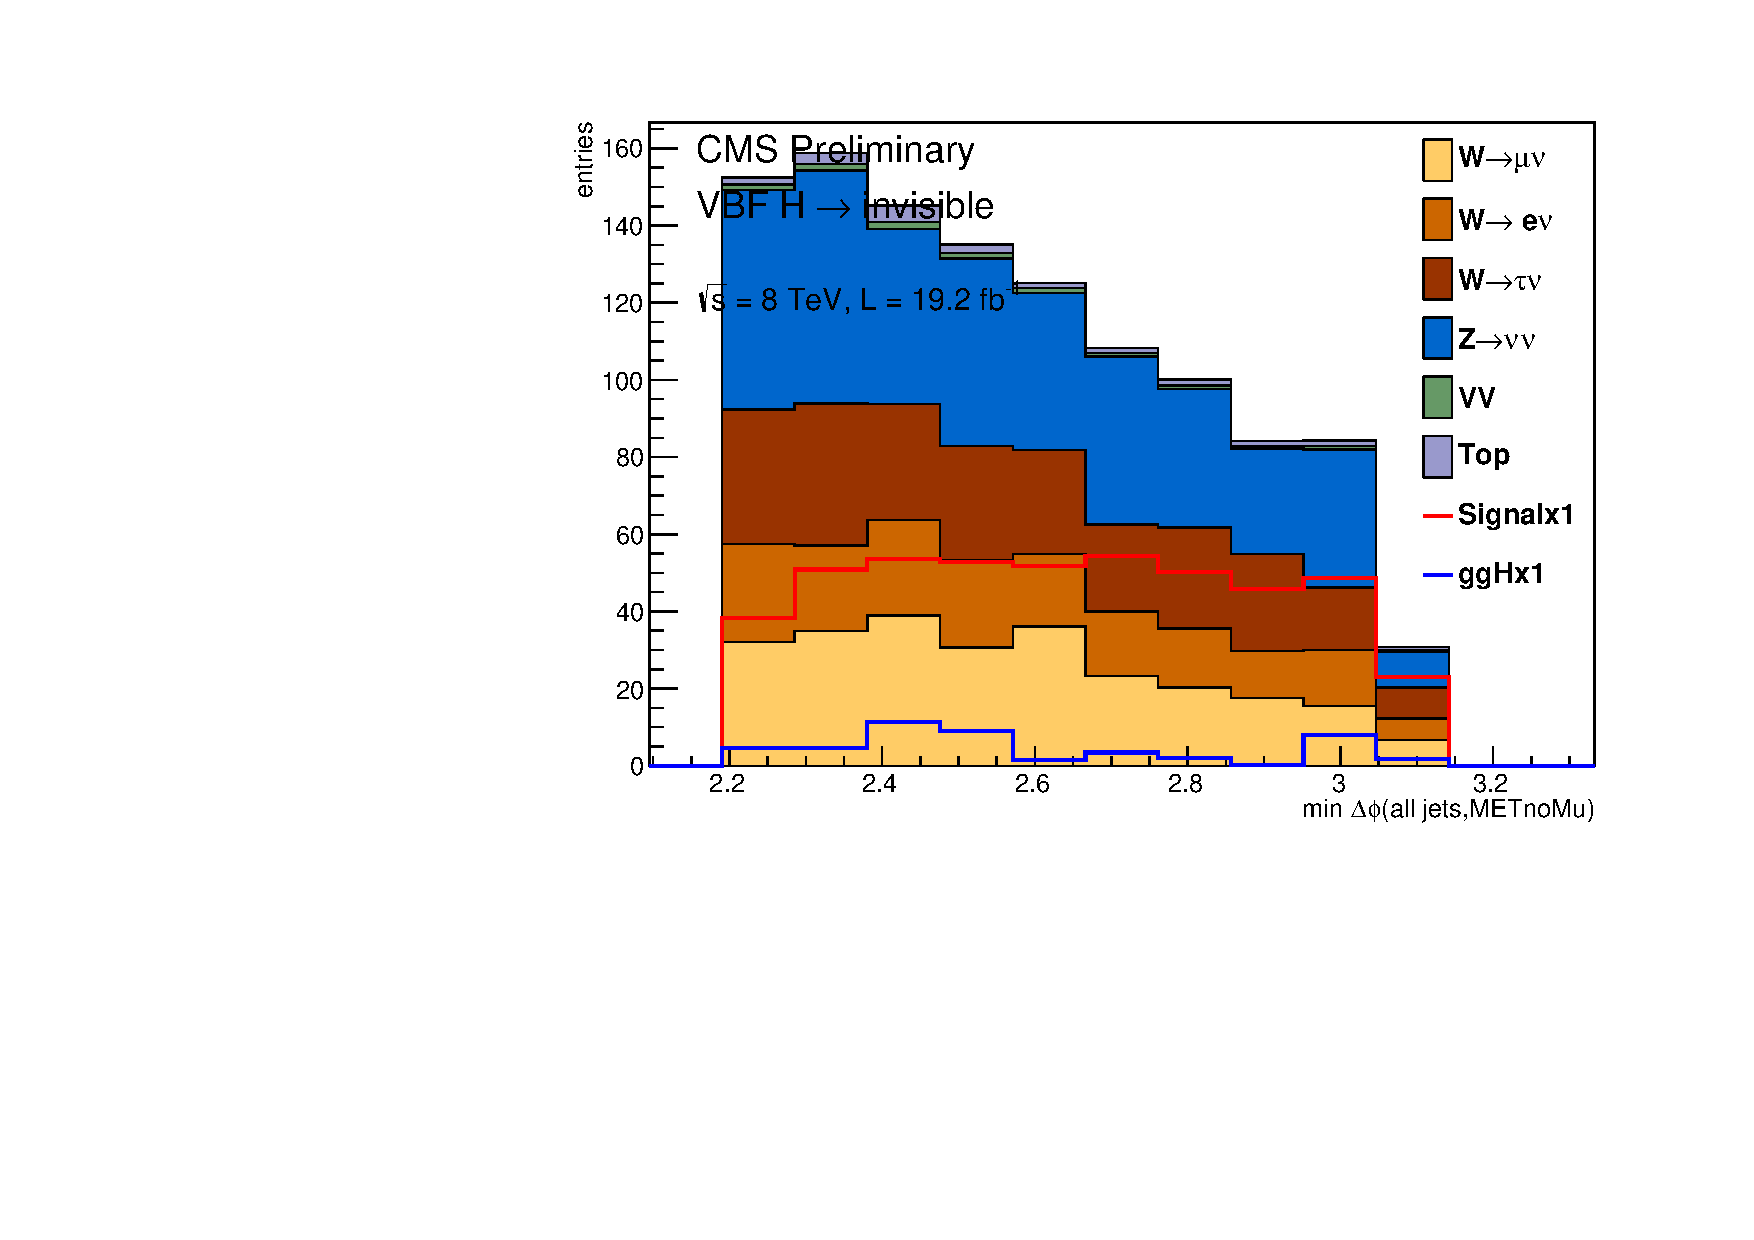
\includegraphics[width=.5\textwidth]{TalkPics/sgs120315/cut.pdf}
    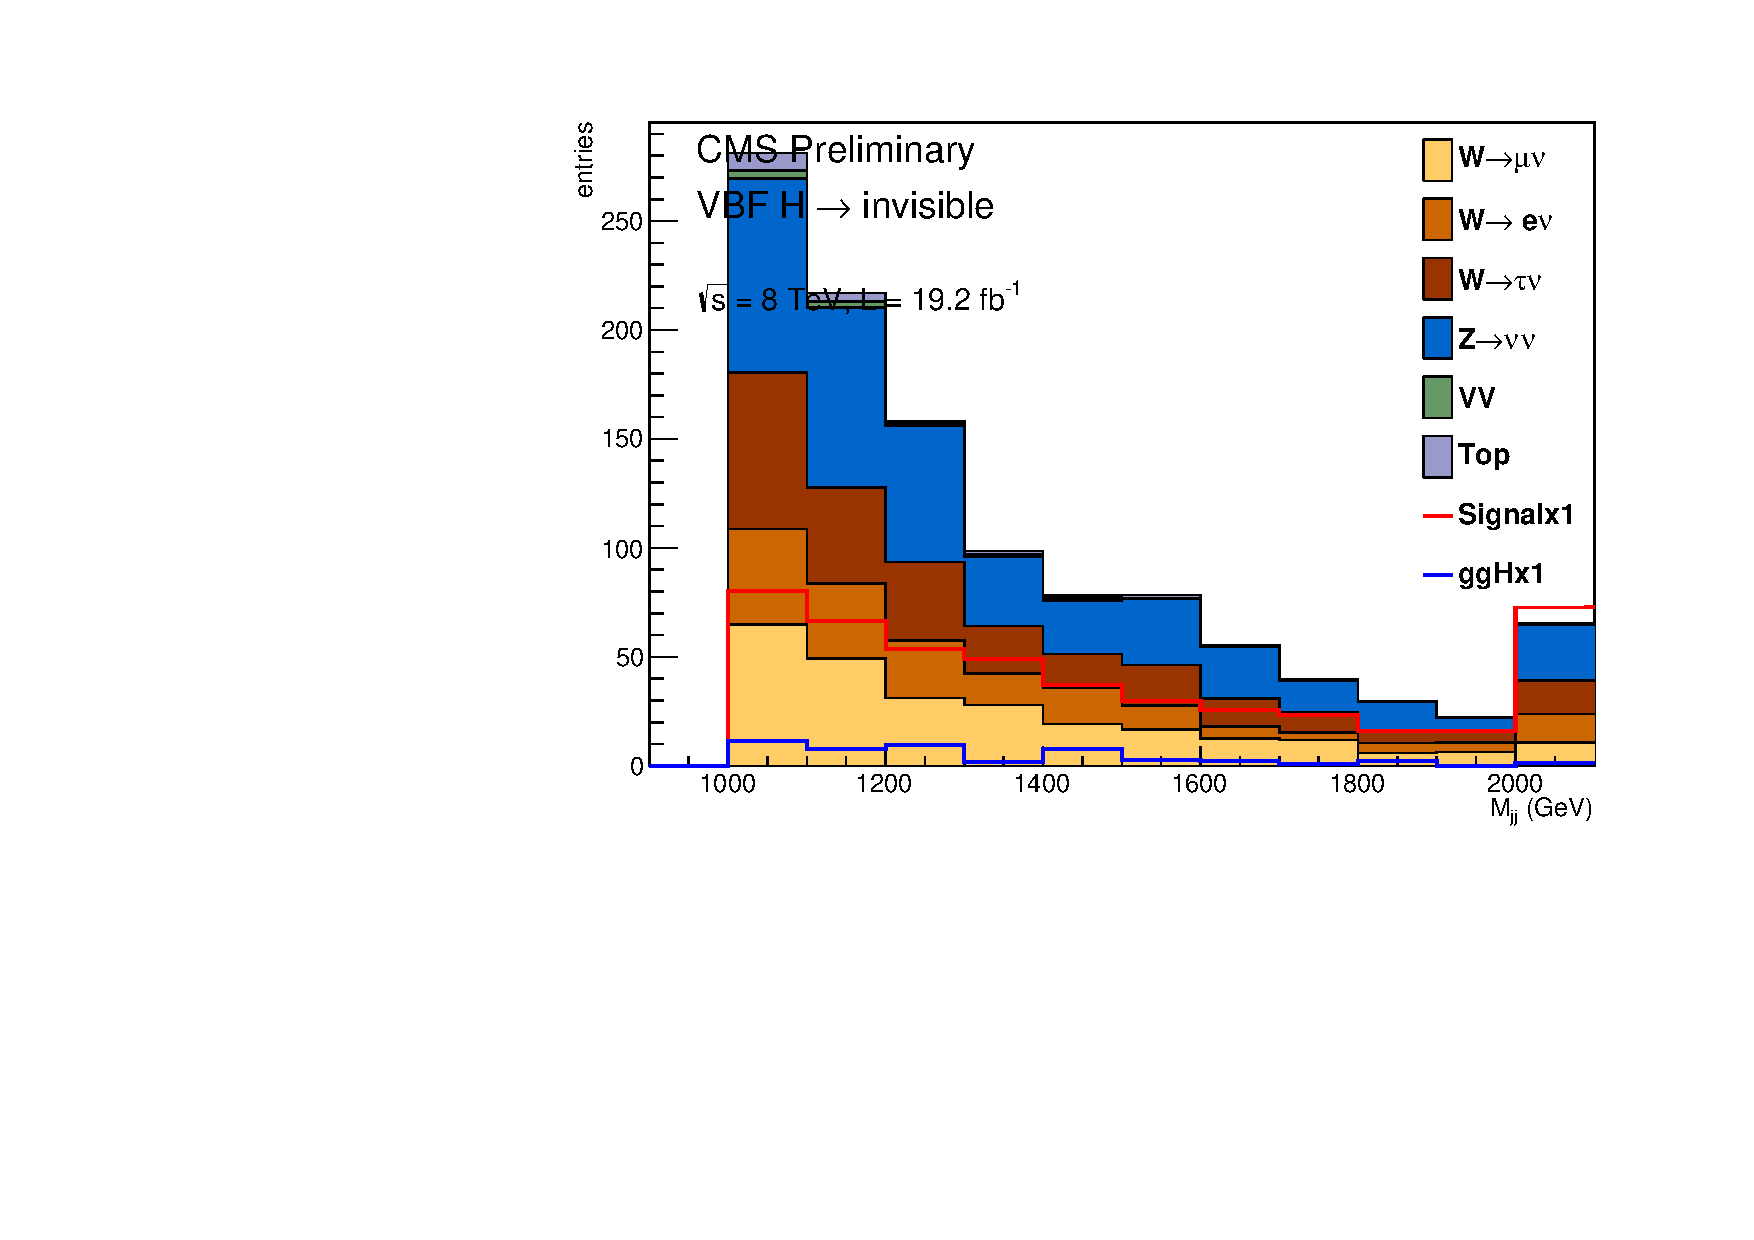
\includegraphics[width=.5\textwidth]{TalkPics/sgs120315/cut2.pdf}
    \begin{itemize}
    \item Predict what you expect to see:
      \begin{itemize}
        \color{beamer@icmiddleblue}
      \item Background only and signal + background
      \end{itemize}
    \end{itemize}
    %!!SOME DISTRIBUTIONS
    %!!LIMIT SETTING
  \end{frame}

  \begin{frame}
    \frametitle{How do we search for it?}
    \begin{itemize}
    \item Compare prediction with data
    \item Use statistics to decide if the result is more like signal or background
    \end{itemize}
    \centering
    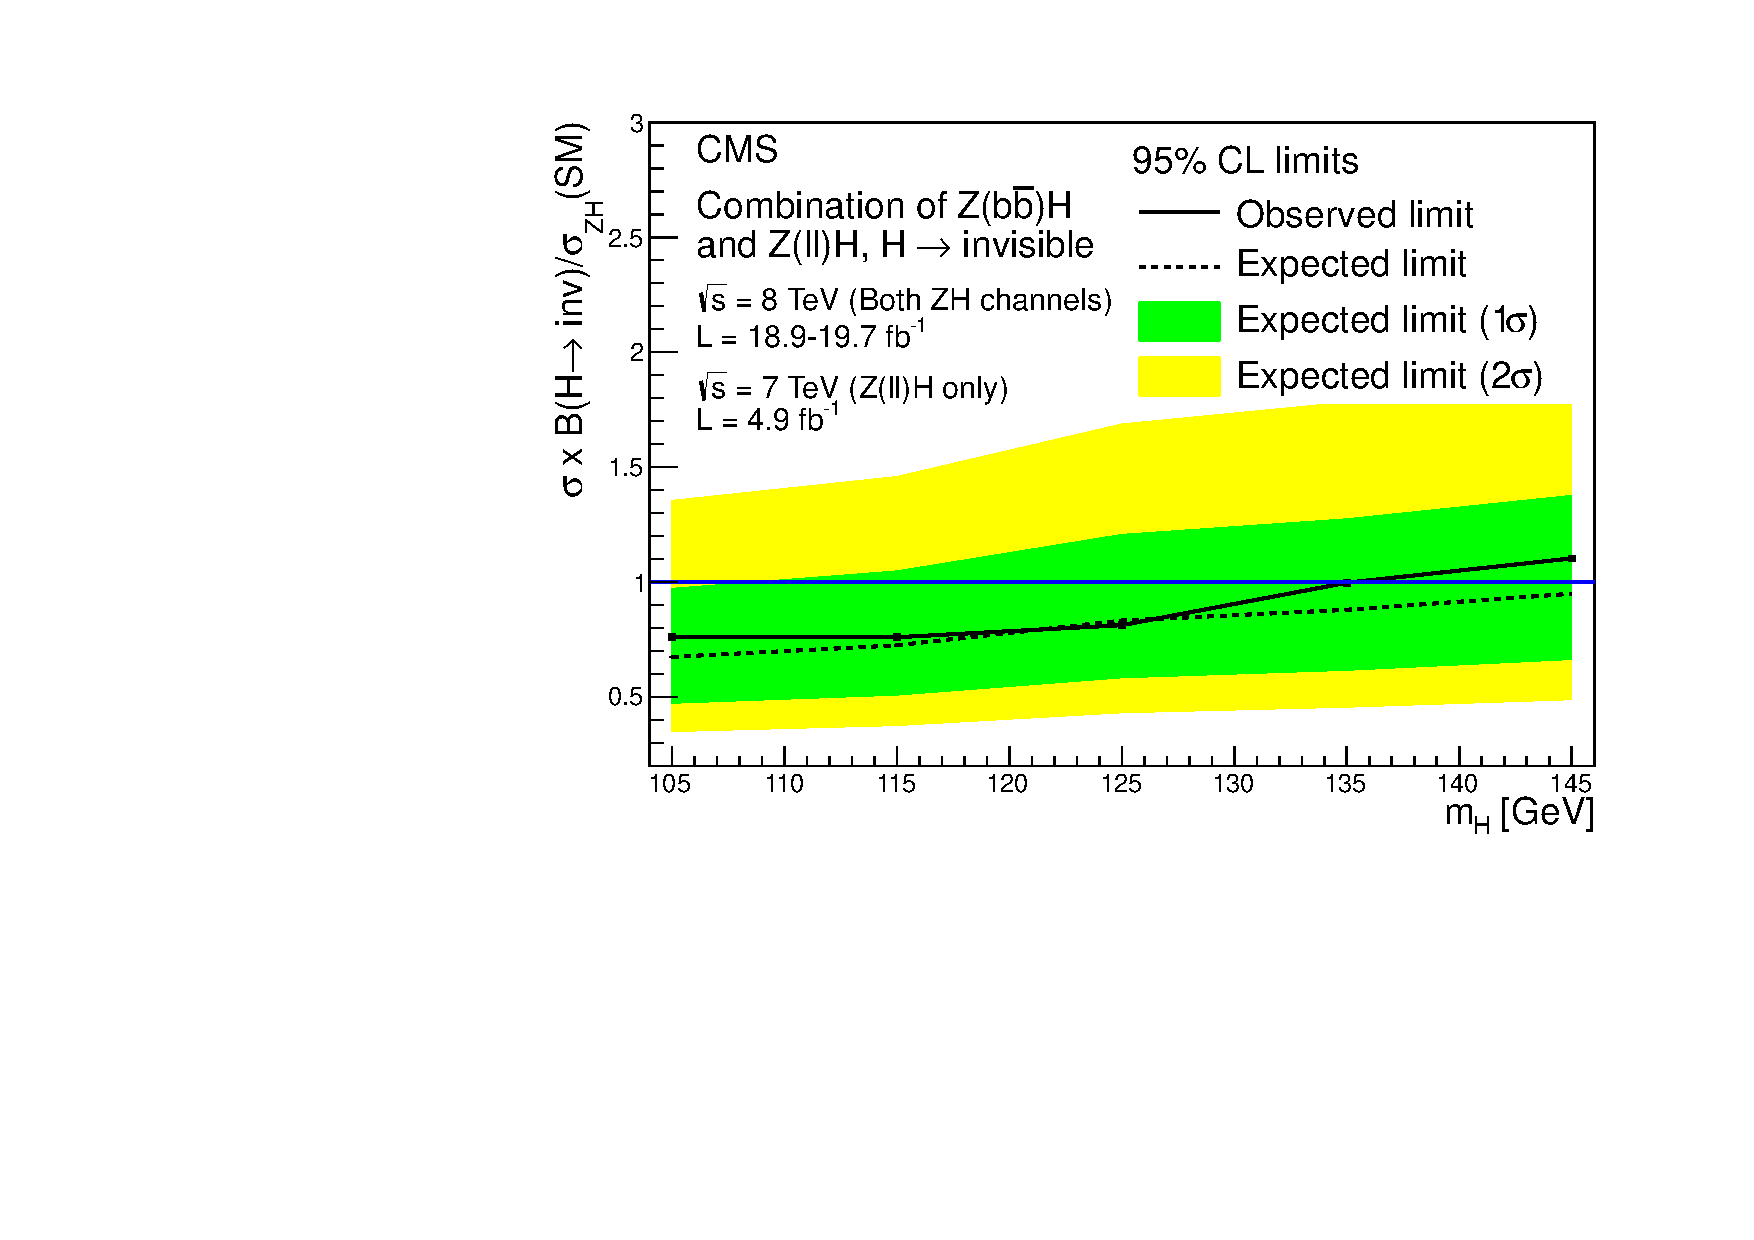
\includegraphics[width=.7\textwidth]{TalkPics/sgs120315/invlimit.pdf}
    %!!LIMIT SETTING
  \end{frame}
  
  \begin{frame}
    \frametitle{What did we find?}
    %!!DISCOVERY LIMITS
    \centering
    \includegraphics[width=.6\textwidth]{../../Reports/Firstyearreport/TalkPics/excdisclowmass.png}
  \end{frame}
  
  \begin{frame}
    \frametitle{Is it a Higgs boson?}
    \begin{itemize}
    \item Not enough to find a new particle:
      \begin{itemize}
        \color{beamer@icmiddleblue}
      \item Higgs boson has very well predicted properties
      \end{itemize}
    \end{itemize}
    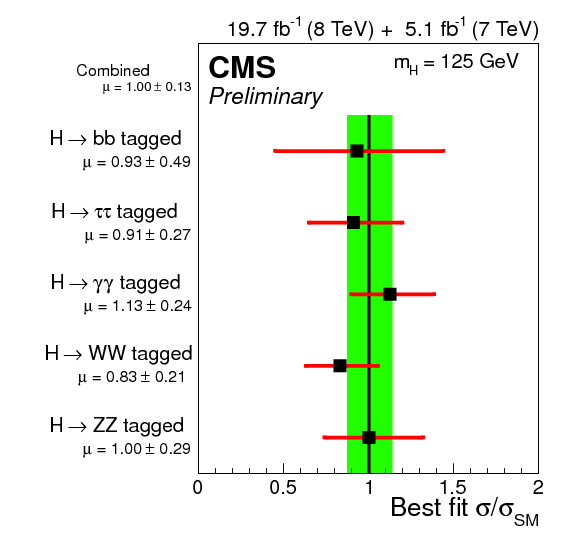
\includegraphics[width=.5\textwidth]{TalkPics/sgs120315/decaybrs.png}
    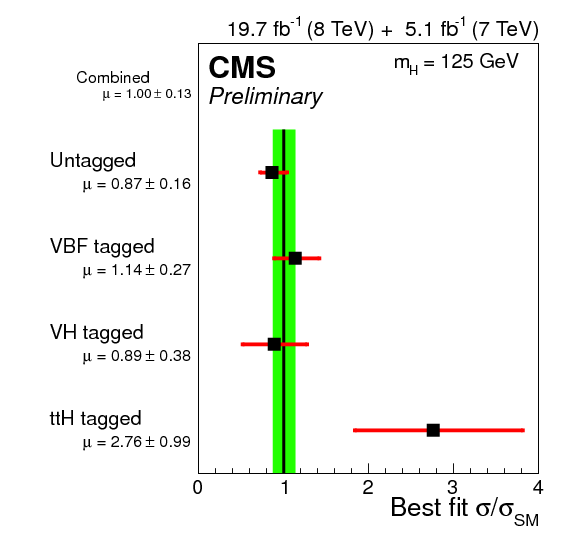
\includegraphics[width=.5\textwidth]{TalkPics/sgs120315/prodbrs.png}
      \end{frame}

  \begin{frame}
    \frametitle{Does it couple to mass?}
    \centering
    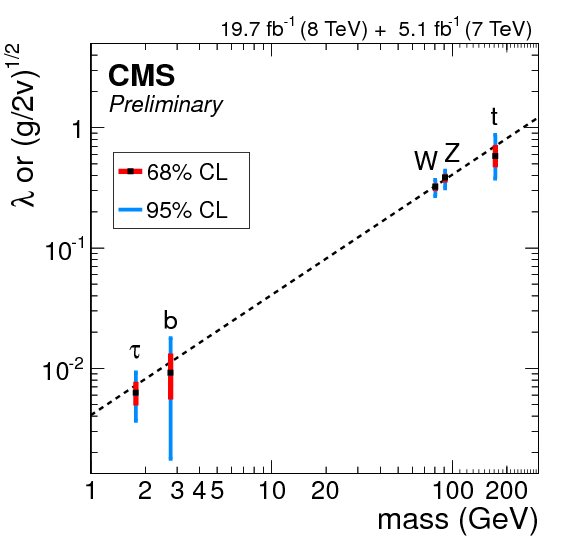
\includegraphics[width=.5\textwidth]{TalkPics/sgs120315/masscoupling.png}
  \end{frame}


  \begin{frame}
    \frametitle{What do we do now?}
    \begin{itemize}
    \item What we see looks very like a Higgs boson:
      \begin{itemize}
        \color{beamer@icmiddleblue}
      \item uncertainties are still large
      \end{itemize}
    \item The SM has problems:
      \begin{itemize}
        \color{beamer@icmiddleblue}
        \item dark matter, fine tuning, matter anti-matter difference, gravity
      \end{itemize}
    \item Many theories try to fix these problems:
      \begin{itemize}
        \color{beamer@icmiddleblue}
        \item these theories often have differently behaving Higgs bosons
      \end{itemize}
    \item Studying the Higgs boson in more detail can confirm/exclude theories
    \end{itemize}
  \end{frame}
  
  \begin{frame}
    \frametitle{What I do: dark matter}
    \begin{itemize}
    \item What is dark matter?
      \begin{itemize}
        \color{beamer@icmiddleblue}
      \item Invisible, cold, massive
      \end{itemize}
    \end{itemize}
    \centering
    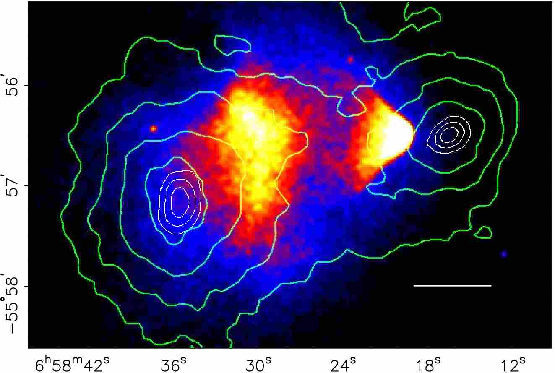
\includegraphics[clip=true,trim=0 0 0 0,height=.5\textheight,width=.5\textwidth]{TalkPics/sgs120315/bulletcluster.png}
      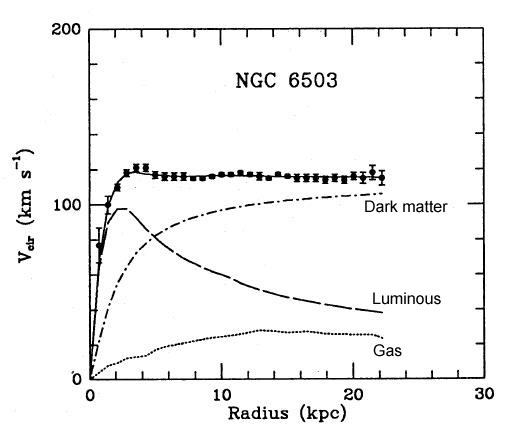
\includegraphics[clip=true,trim=0 0 0 0,height=.53\textheight,width=.5\textwidth]{TalkPics/sgs120315/rotationcurve.jpg}
      %!!PROBLEMS WITH THE SM
      %!!MUST STUDY WHAT WE KNOW IN DETAIL TO LOOK FOR DEVIATIONS AND LOOK FOR NEW PARTICLES
      
      
  \end{frame}

  \begin{frame}
    \frametitle{Why is the Higgs boson a good place to look for dark matter}
    \begin{itemize}
    \item If dark matter has mass it should couple to the Higgs
    \item If it's light enough the Higgs will decay to it
    \item Look for invisibly decaying Higgs...
    \end{itemize}
    \centering
    
\includegraphics[width=.5\textwidth]{TalkPics/sgs120315/question.jpg}
  \end{frame}

  \begin{frame}
    \frametitle{Finding something invisible}
    \begin{itemize}
    \item Higgs must be created with something else
      \begin{itemize}
        \color{beamer@icmiddleblue}
      \item VBF, ZH
      \end{itemize}
    \end{itemize}
    \centering
    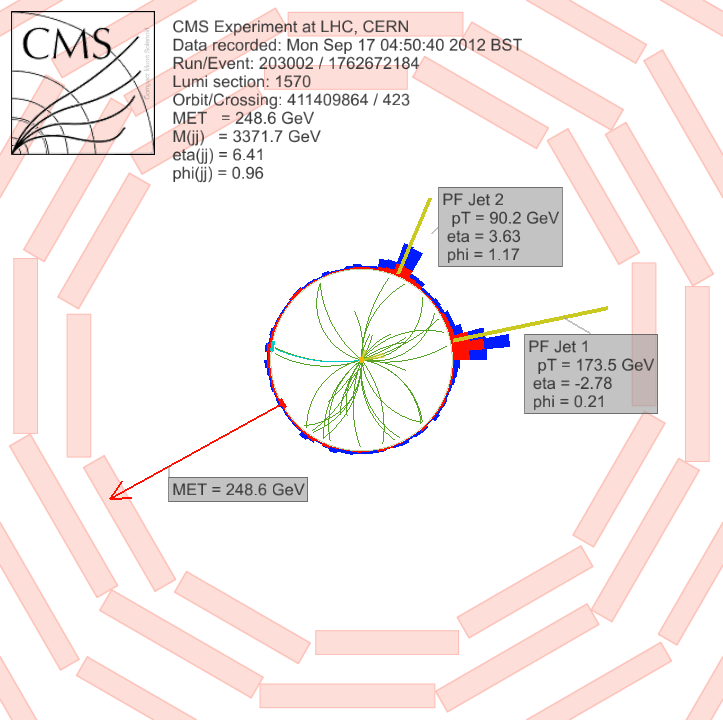
\includegraphics[width=.5\textwidth]{TalkPics/sgs120315/vbfevent.png}
  \end{frame}

  \begin{frame}
    \frametitle{What do we see?}
    \begin{itemize}
    \item Invisible decays very rare in SM
      \begin{itemize}
        \color{beamer@icmiddleblue}
      \item if we see anything it's very likely to be dark matter
      \end{itemize}
    \end{itemize}
    \centering
    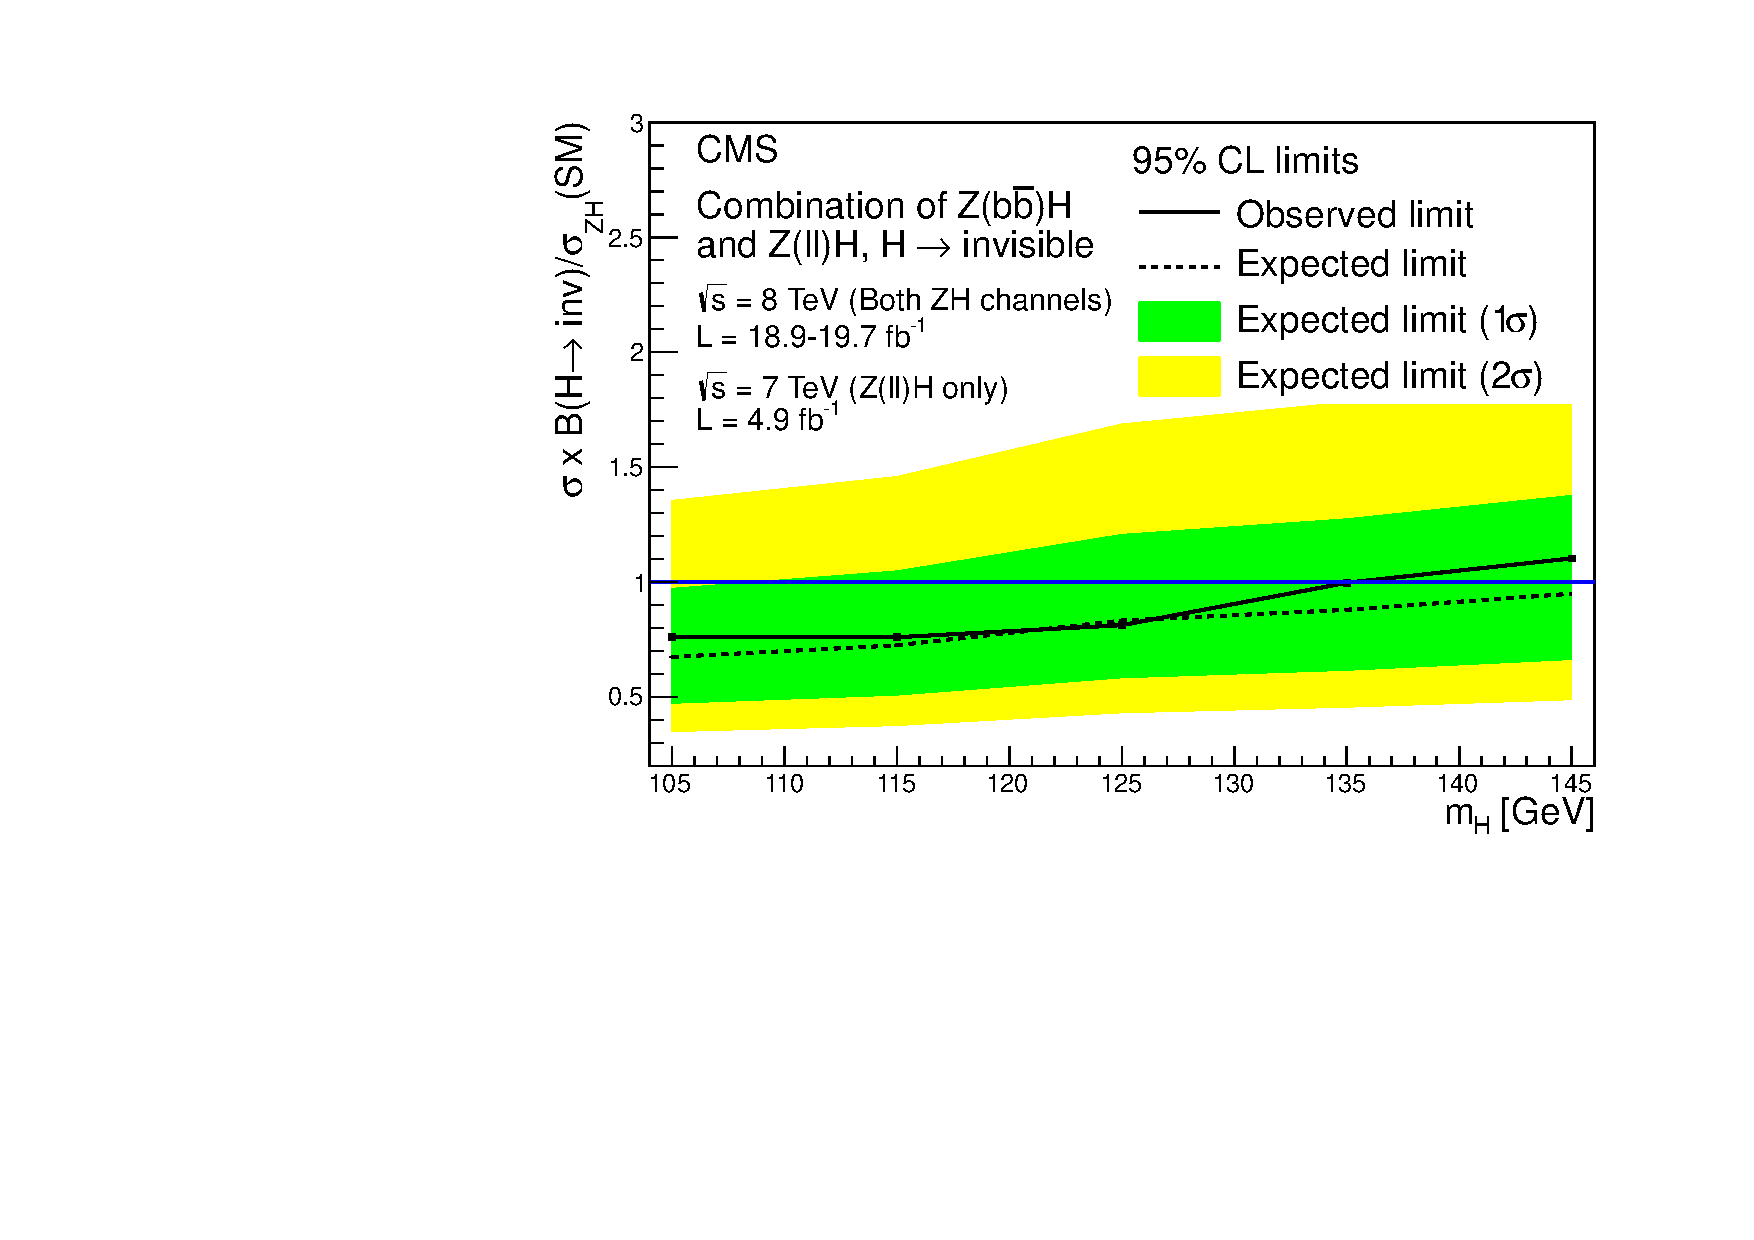
\includegraphics[width=.7\textwidth]{TalkPics/sgs120315/invlimit.pdf}    
  \end{frame}

  \begin{frame}
    \frametitle{Summary}
    \label{lastframe}
    \begin{itemize}
    \item The Higgs boson gives mass to all the particles we know about
    \item We found something which looks very like it at the LHC
    \item Discovery is only the beginning
      \begin{itemize}
        \color{beamer@icmiddleblue}
      \item the Higgs boson might tell us how to fix the SM
      \item some theories predict 5 Higgs bosons!
      \end{itemize}
    \end{itemize}
    \centering
    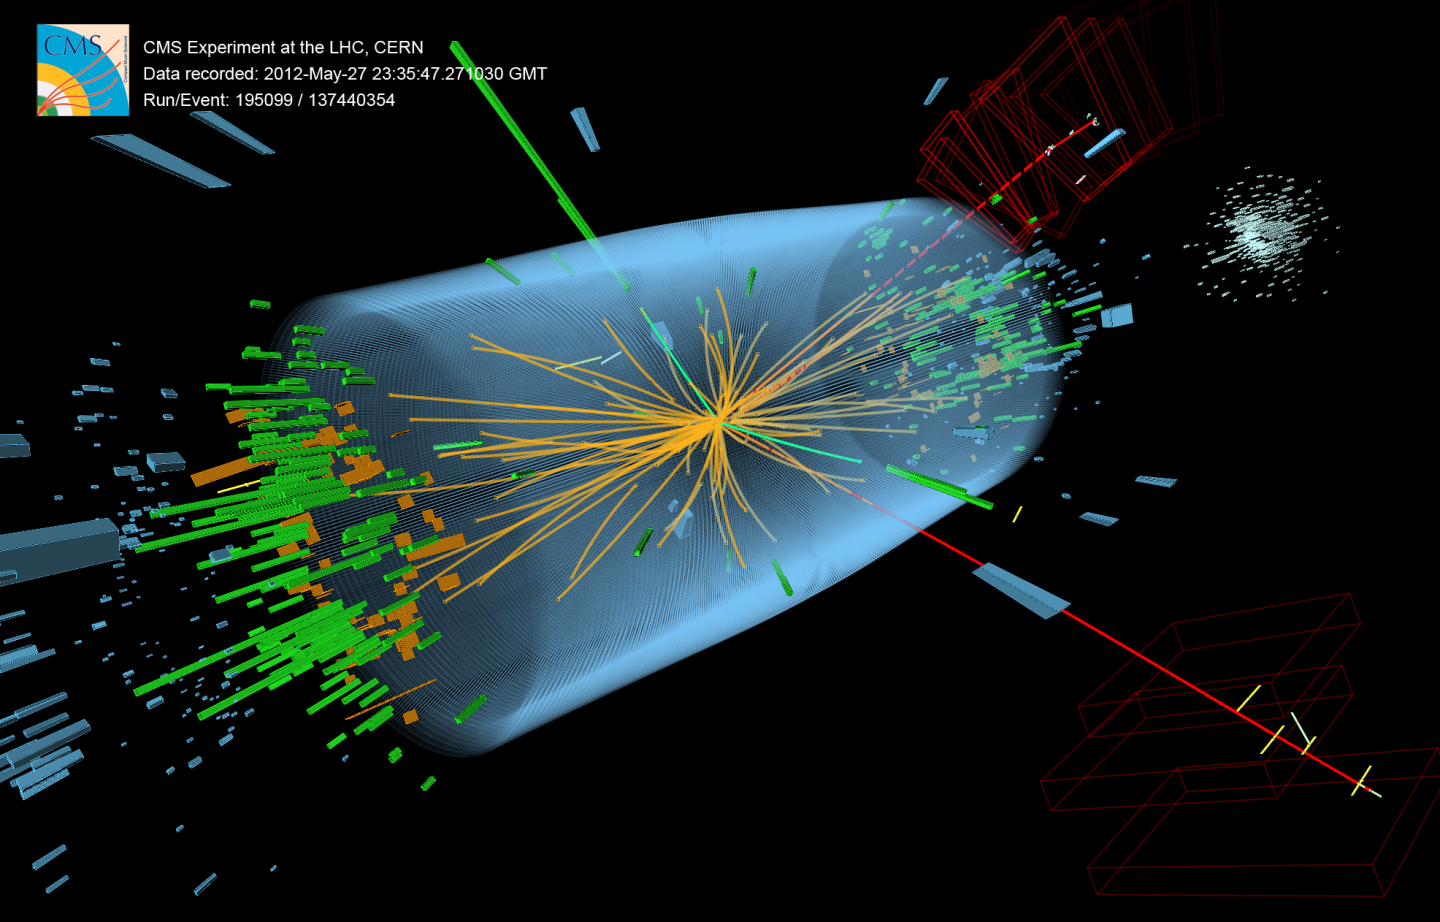
\includegraphics[width=.5\textwidth]{TalkPics/sgs120315/eventdisplay.png}
  \end{frame}
  
  %HIGGS BACKGROUND
  \begin{frame}
    \frametitle{The Higgs Boson}
    \begin{columns}
      \column{.5\textwidth}

      \column{.5\textwidth}

    \end{columns}
  \end{frame}

  \begin{frame}
    \frametitle{What do I do?}
    \centering
    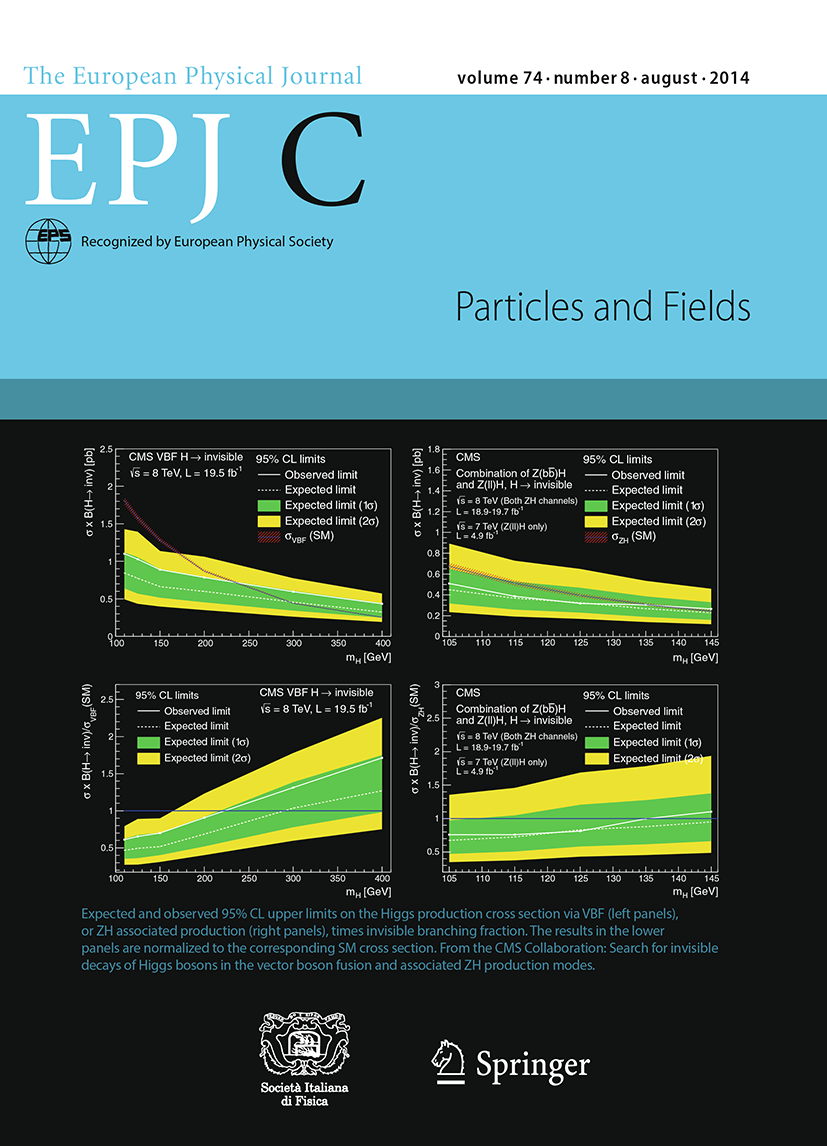
\includegraphics[height=.85\textheight]{TalkPics/EPJCAug2014Cover.png}
  \end{frame}

  \begin{frame}
    \frametitle{Why Higgs to Invisible?}
    \vspace{-.2cm}
    \begin{columns}
      \column{.5\textwidth}
      \begin{block}{\scriptsize Experimental motivation}
        \scriptsize
        \begin{itemize}
        \item Current measurements of the 125 GeV Higgs boson are compatible with Standard Model (SM) expectations
        \item[-] large uncertainties can still accommodate significant beyond the SM (BSM) properties
        \item Additional Higgs bosons with exotic decays are not excluded
        \end{itemize}
      \end{block}
      \column{.45\textwidth}
      \hfill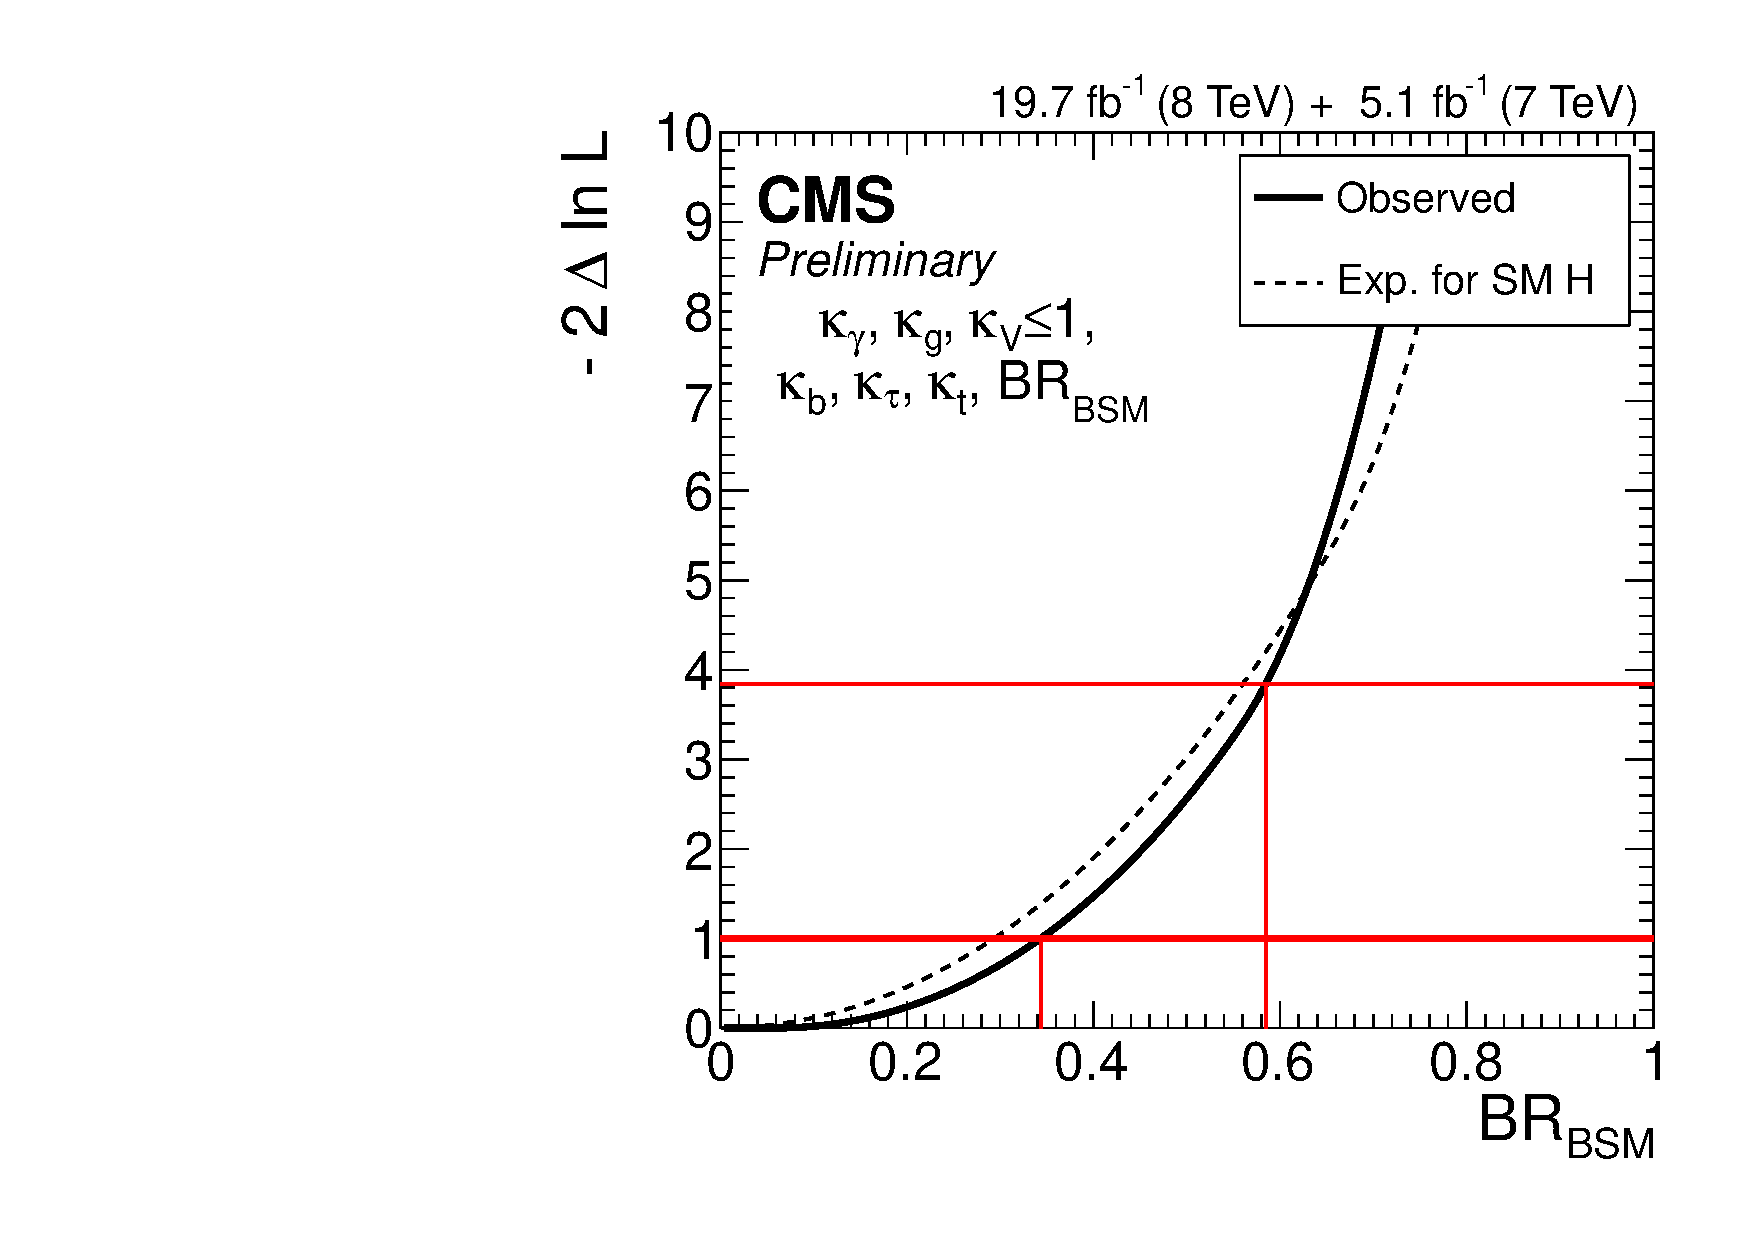
\includegraphics[height=.55\textheight]{TalkPics/panicpics/indirectbrbsm.pdf}
      \column{.05\textwidth}
      \begin{turn}{-90}\scriptsize CMS-PAS-HIG-14-009\end{turn}
    \end{columns}
    \begin{columns}
      \column{1.095\textwidth}
      \begin{block}{\scriptsize Theoretical motivation}
        \scriptsize
        \begin{itemize}
        \item Many BSM theories predict Higgs boson decays to invisible final states:
        \item[-] e.g. SUSY, extra dimensions, fourth-generation neutrinos
        \item These final state particles are often dark matter candidates
        \end{itemize}
      \end{block}
    \end{columns}

  \end{frame}

  %!!SIMPLIFY ALL FROM HERE
  %!!EXPLAIN DATA FLOW AND HOW TO DO AN ANALYSIS

\end{fmffile}
\end{document}

